\documentclass[12pt,a4paper,titlepage,listof=totoc,bibliography=totoc,chapteratlists=0pt]{scrreprt}

\begin{filecontents*}{\jobname.xmpdata}
	\Keywords{VR, IOT, TODO}
	\Title{Unser tolles Thema -- wir sind suppa}
	\Author{Stefan Schwammal, Susi Schwammal}
\end{filecontents*}

\setcounter{tocdepth}{1}

\usepackage[utf8]{inputenc}
\usepackage[T1]{fontenc}
\usepackage{amsmath}
\usepackage{amsfonts}
\usepackage{amssymb}
\usepackage[table]{xcolor}
\usepackage{graphicx}
\usepackage[left=3.50cm, right=2.00cm, top=2.00cm, bottom=2.00cm,foot=1cm]{geometry}
\usepackage[splitrule,hang,flushmargin,multiple,bottom]{footmisc}
\usepackage{lmodern, textcomp}
\usepackage{lmodern}
\usepackage{pdfpages}
\usepackage[ngerman]{babel}
\usepackage{multicol}
\usepackage{subfig}
\usepackage{float}
\usepackage{array,tabularx,booktabs}
\usepackage{ragged2e}
\usepackage{lipsum}
\usepackage{wrapfig}

\newcolumntype{M}[1]{>{\centering\arraybackslash}m{#1}}

\usepackage{enumitem}
\newlist{compactitem}{itemize}{3}
\setlist[compactitem,1]{label=\textbullet, nosep,leftmargin=1.5em,labelwidth=*,align=left}
\setlist[compactitem,2]{label=--, nosep,leftmargin=1.5em,labelwidth=*,align=left}
\setlist[compactitem,3]{label=\textopenbullet, nosep,leftmargin=1.5em,labelwidth=*,align=left}
\newlist{compactenum}{enumerate}{3}
\setlist[compactenum,1]{label=\arabic*., nosep,leftmargin=1.5em,labelwidth=*,align=left}
\setlist[compactenum,2]{label=\alph*., nosep,leftmargin=1.5em,labelwidth=*,align=left}
\setlist[compactenum,3]{label=\roman*., nosep,leftmargin=1.5em,labelwidth=*,align=left}
\newlist{compactdesc}{description}{3}
\setlist[compactdesc]{leftmargin=1.5em,labelwidth=*,align=left}

\usepackage{microtype}

\usepackage[parfill]{parskip}

\definecolor{bluekeywords}{rgb}{0.13,0.13,1}
\definecolor{greencomments}{rgb}{0,0.5,0}
\definecolor{redstrings}{rgb}{0.9,0,0}
\definecolor{lightgray}{gray}{0.9}
\definecolor{lightblue}{rgb}{0.93,0.95,1.0}

\usepackage{listings}

\makeatletter
\lstdefinestyle{lststyle}{
	basicstyle=%
	\ttfamily
	\lst@ifdisplaystyle\scriptsize\fi
}
\makeatother

\renewcommand{\lstlistlistingname}{List of Listings}
% TODO: define other languages as needed
\lstset{language=Python,
numbers=left,               
numberstyle=\tiny,          
showspaces=false,
showtabs=false,
breaklines=true,
lineskip=-1pt,
tabsize=2,
showstringspaces=false,
breakatwhitespace=true,
escapeinside={(*@}{@*)},
commentstyle=\color{greencomments},
keywordstyle=\color{bluekeywords}\bfseries,
stringstyle=\color{redstrings},
style=lststyle,
xleftmargin=17pt,
         framexleftmargin=17pt,
         framexrightmargin=5pt,
         framexbottommargin=4pt
}
\lstset{
morekeywords={base,var,in,out,dynamic,from,where,select,orderby,function,\$,group,by,into,yield,async,await,@,None,self,as,elif,with}
}
\lstdefinelanguage{TypeScript}{
	keywords={typeof, new, true, false, catch, function, return, null, switch, var, if, in, while, do, else, case, break, void, number, string, boolean, module, \$, export, for, this},
	keywordstyle=\color{blue}\bfseries,
	ndkeywords={class, export, boolean, throw, implements, import, this},
	ndkeywordstyle=\color{darkgray}\bfseries,
	identifierstyle=\color{black},
	sensitive=false,
	comment=[l]{//},
	morecomment=[s]{/*}{*/},
	commentstyle=\color{purple}\ttfamily,
	stringstyle=\color{red}\ttfamily,
	morestring=[b]',
	morestring=[b]"
}
\usepackage{caption}
\DeclareCaptionFont{white}{\color{white}}
\DeclareCaptionFormat{listing}{\colorbox[cmyk]{0.43, 0.35, 0.35,0.01}{\parbox{\textwidth}{\hspace{10pt}#1#2#3}}}
\captionsetup[lstlisting]{format=listing,labelfont=white,textfont=white} 
\captionsetup[table]{justification=centering, singlelinecheck=false}

\usepackage{setspace}
\newcommand{\MSonehalfspacing}{%
	\setstretch{1.44}%  default
	\ifcase \@ptsize \relax % 10pt
	\setstretch {1.448}%
	\or % 11pt
	\setstretch {1.399}%
	\or % 12pt
	\setstretch {1.433}%
	\fi
}

\newcommand{\setauthor}[1]{\ohead[]{#1}}

\usepackage[automark]{scrlayer-scrpage}
\pagestyle{scrheadings}
\automark{chapter}
\renewcommand\sectionmark[1]{\markright{\MakeMarkcase {\thesection\hskip .5em\relax#1}}}
\rohead{\ifnum\expandafter\pdfstrcmp\botmark=0 \rightmark\else\leftmark{} --- \rightmark\fi}
\ihead[]{\headmark}
\chead[]{}
\ohead{}
\cfoot[]{}
\ofoot[\pagemark]{\pagemark}
\setheadsepline{.1pt}

\usepackage[hyphens]{url}

\usepackage[a-1b]{pdfx}

\usepackage{hyperref}
\hypersetup{pdfa}

\usepackage[nonumberlist,toc,nopostdot]{glossaries}

\usepackage{chngcntr}
\counterwithout{footnote}{chapter}
\counterwithout{figure}{chapter}
\counterwithout{table}{chapter}
\AtBeginDocument{
	\counterwithout{lstlisting}{chapter}
	\urlstyle{sf}
}
\newcounter{RPages}

\makeatletter
\def\bstctlcite{\@ifnextchar[{\@bstctlcite}{\@bstctlcite[@auxout]}}
\def\@bstctlcite[#1]#2{\@bsphack
	\@for\@citeb:=#2\do{%
		\edef\@citeb{\expandafter\@firstofone\@citeb}%
		\if@filesw\immediate\write\csname #1\endcsname{\string\citation{\@citeb}}\fi}%
	\@esphack}
\makeatother

\clubpenalty=10000
\widowpenalty=10000
\displaywidowpenalty=10000
\interfootnotelinepenalty=10000

\title{LeoTour}
\author{Oliver Sugic}

\makeindex
\makeglossaries
\begin{document}
\bstctlcite{IEEEexample:BSTcontrol}
\newcommand{\reminder}[1]
{ \textcolor{red}{<[{\bf\marginpar{\mbox{$<==$}} #1 }]>} }
\newcommand{\icode}[1]{\lstinline$#1$}
%\urlstyle{same}
%\setstretch{1.5}
\setstretch {1.433}
\renewcommand{\arraystretch}{1.2}

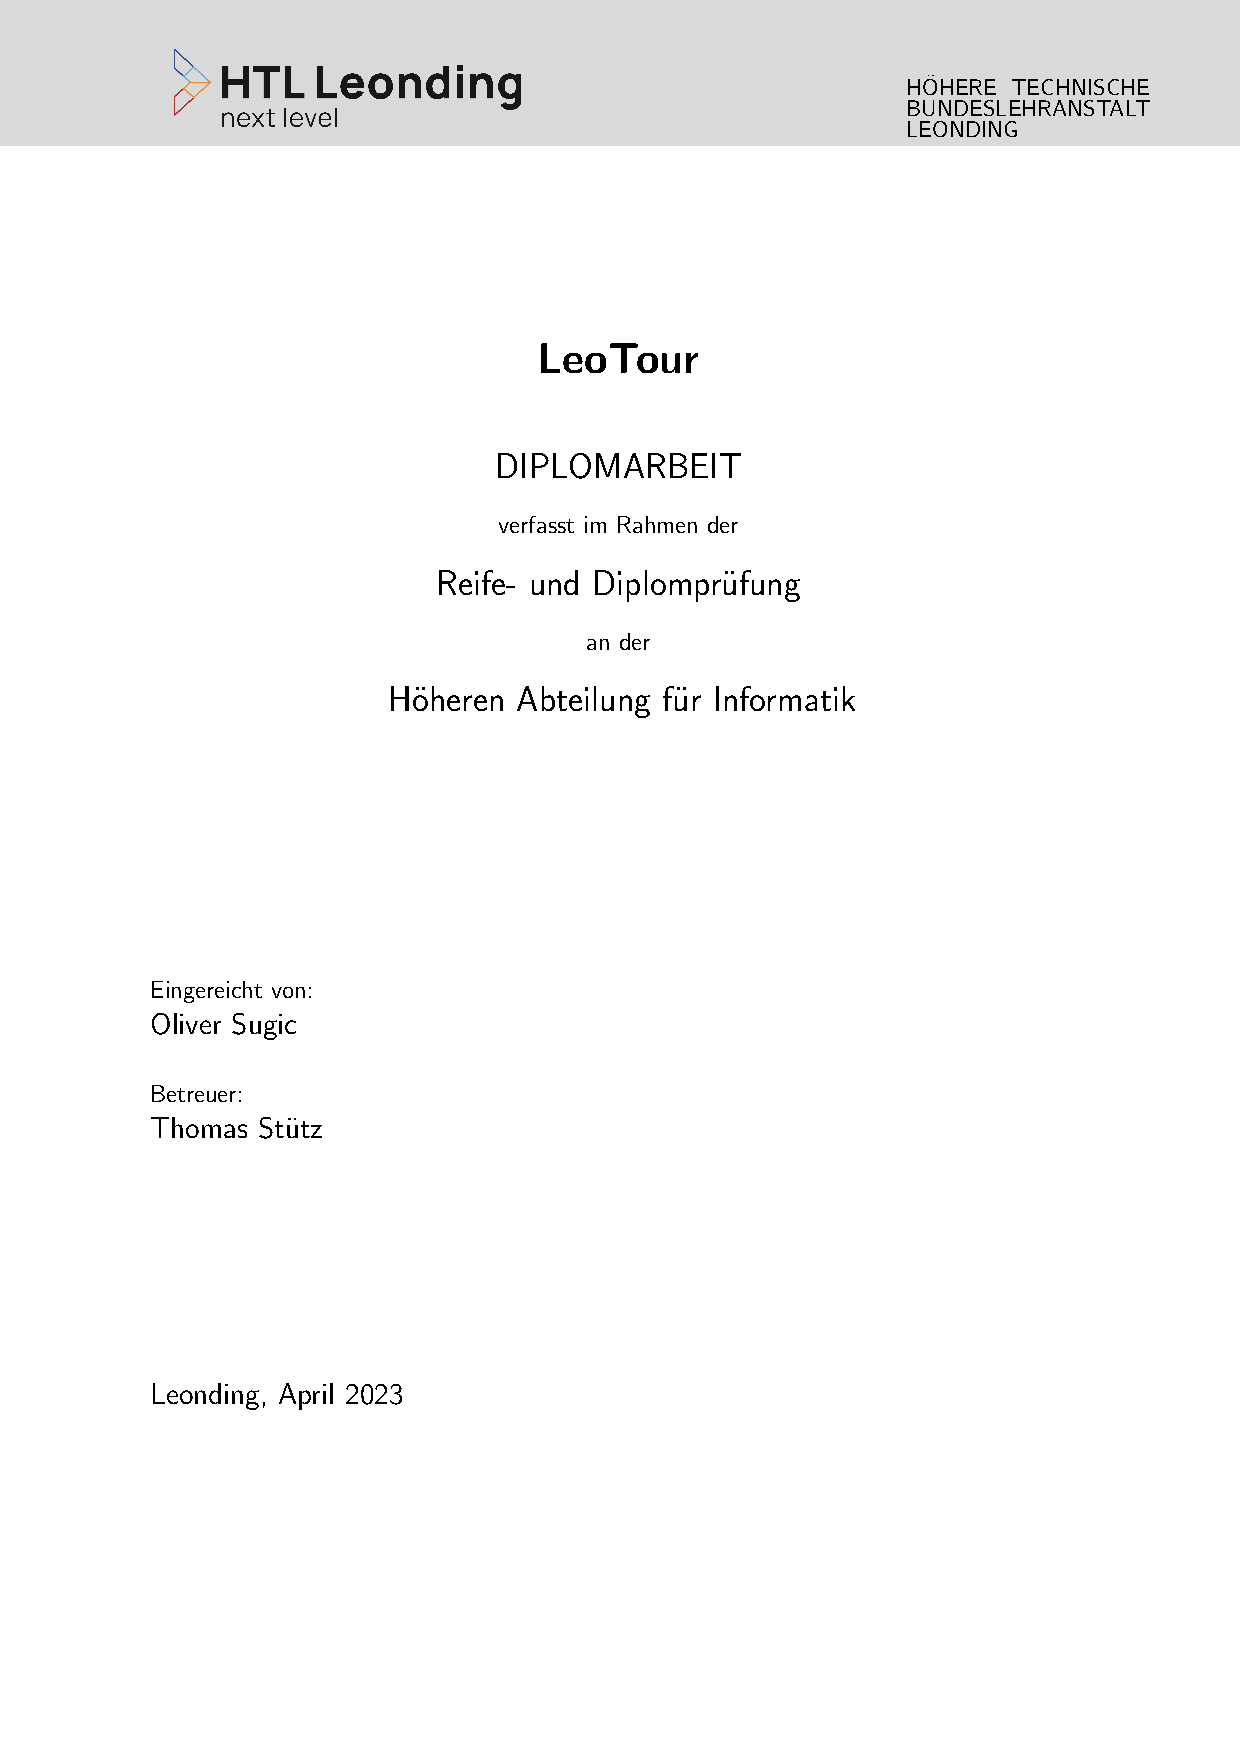
\includepdf{./titlepage/coversheet}
\pagenumbering{Roman}
\newpage
\thispagestyle{empty}
\vspace{3cm}
~ \\ \\
Ich erkläre an Eides statt, dass ich die vorliegende Diplomarbeit selbstständig und ohne fremde Hilfe verfasst, andere als die angegebenen Quellen und Hilfsmittel nicht benutzt bzw. die wörtlich oder sinngemäß entnommenen Stellen als solche kenntlich gemacht habe.

Die Arbeit wurde bisher in gleicher oder ähnlicher Weise keiner anderen Prüfungsbehörde vorgelegt und auch noch nicht veröffentlicht.

Die vorliegende Diplomarbeit ist mit dem elektronisch übermittelten Textdokument identisch.
\vspace{3cm}
% Hier kommt die Unterschrift drüber
\begin{tabbing}
Leonding, April 2023 \hspace{5cm} Oliver Sugic
\end{tabbing}
\vspace{10cm}
\newpage
\setcounter{page}{1}

\begin{spacing}{1}
    \chapter*{Abstract}
\end{spacing}
\begin{wrapfigure}{r}{0.3\textwidth}
    \begin{center}
      
\includegraphics[width=0.2\textwidth]{pics/question_mark.png}
    \end{center}
\end{wrapfigure}
Brief summary of our amazing work. In English.
This is the only time we have to include a picture within the text.
The picture should somehow represent your thesis.
This is untypical for scientific work but required by the powers that are.
\lipsum[6]
\newpage
\begin{spacing}{1}
    \chapter*{Zusammenfassung}
\end{spacing}
\begin{wrapfigure}{r}{0.3\textwidth}
    \begin{center}
      
\includegraphics[width=0.2\textwidth]{pics/question_mark.png}
    \end{center}
\end{wrapfigure}
Zusammenfassung unserer genialen Arbeit. Auf Deutsch.
Das ist das einzige Mal, dass eine Grafik in den Textfluss eingebunden wird.
Die gewählte Grafik soll irgendwie eure Arbeit repräsentieren.
Das ist ungewöhnlich für eine wissenschaftliche Arbeit aber eine Anforderung der Obrigkeit.
\emph{Bitte auf keinen Fall mit der Zusammenfassung verwechseln, die den Abschluss der Arbeit bildet!}
\lipsum[6]


\pagestyle{plain}

\renewcommand{\lstlistlistingname}{Quellcodeverzeichnis}

\tableofcontents
\newpage
\setcounter{RPages}{\value{page}}
\setcounter{page}{0}
\pagenumbering{arabic}
\pagestyle{scrheadings}

\begin{spacing}{1}
\chapter{Ausgangssituation und Zielsetzung}\label{chapter:introduction}
\end{spacing}
\section{Ausgangssituation}
\setauthor{Oliver Sugic}
An der HTBLA Leonding befinden etwa 1000 Schüler und 100 Lehrer.
Die Schüler fahren auf Exkursionen wie z.B Sportwochen im Ausland oder auch im Inland.

\section{Ist-Zustand}
\setauthor{Oliver Sugic}
Derzeit werden viele Exkursionen in unbekannte Gebiete unternommen. Es wird mehr Lehrpersonal mitgenommen um so besser auf Schüler und Schülerinnen aufzupassen und den Überblick zu behalten. Dies ist jedoch sehr aufwendig und kostspielig. 

\section{Beschreibung der Problemstellung}
\setauthor{Oliver Sugic}
In einer großen Gruppe mit oftmals mehreren Lehrern und Lehrerinnen ist es schwierig, die Schüler zu organisieren und zu kontrollieren und  den Überblick zu behalten. Die Lehrern und Lehrerinnen müssen sich um die Schüler und Schülerinnen kümmern da diese oftmals nicht aufmerksam sind und sich leicht verirren können oder auch von der sich von der Gruppe trennen ohne es zu merken.

Oft werden Informationen über die Exkursionen nur mündlich weitergegeben und es gibt keine Möglichkeit diese Informationen nachzulesen. Außerdem kann es passieren, dass die Schüler und Schülerinnen die Informationen nicht richtig verstanden haben oder auch die Informationen nicht richtig weitergegeben wurden.

\newpage

\section{Marktanalyse}
\setauthor{Oliver Sugic}
Um eine fertige Produkt zu verwenden musste eine Marktanalyse durchgeführt werden. Es wurden verschiedene Produkte verglichen und analysiert. Dabei wurden die folgenden Kriterien betrachtet:
\begin{itemize}
    \item Funktionalität: Wie einfach können Reisen geplant werden? 
    \item Benutzerfreundlichkeit: Wie einfach ist die Bedienung für die Teilnehmer der Reise?
    \item Preis: Wie viel kostet das Produkt?
    \item Datenschutz: Wie sicher sind die Daten der Teilnehmer der Reise? Werden Standortdaten gespeichert?
\end{itemize}

\subsection{Wanderlog}
\setauthor{Oliver Sugic}
\cite{Sewell} Wanderlog ist eine mobile App des Unternehmens Travelchime Inc. .Mit dieser App können Reisen geplant und durchgeführt werden. Die App ist kostenlos und kann für Android und iOS heruntergeladen werden. Die App bietet Funktionen wie Planung und Verbesserungen von Reisepläne. Mit der Pro-Version ist es möglich die Route der Reise zu optimieren um Geld zu sparen, als auch die Nutzung der App offline zu ermöglichen. Die Nutzung der Pro-Version kostet allerdings 49.99\$ jährlich


\subsection{TripIt}
\setauthor{Oliver Sugic}
TripIt ist eine mobile App des Unternehmens Concur Technologies. Durch die Möglichkeiten der App kann die Organisation und Verw
\cite{}

\section{Aufgabenstellung}
\setauthor{Oliver Sugic}


\begin{spacing}{2}
\subsection{Gesamtkonzept}
\setauthor{Oliver Sugic}
\end{spacing}

\begin{spacing}{2}
\subsection{Aufgabenbereiche der vorliegenden Arbeit}
\setauthor{Oliver Sugic}
\end{spacing}

\begin{spacing}{2}
\subsection{Funktionale Anforderungen}
\setauthor{Oliver Sugic}
\end{spacing}

\begin{spacing}{2}
\subsection{Nicht funktionale Anforderungen}
\setauthor{Oliver Sugic}
\end{spacing}

\begin{spacing}{2}
\section{Ziele}
\setauthor{Oliver Sugic}
\end{spacing}
    


\begin{spacing}{1}
\chapter{Systemarchitektur}
\end{spacing}
\section{Verschiedene Versionen der Anzeige}
\setauthor{Oliver Sugic}
Für die graphische Oberfläche wurden verschiedene Ideen und Konzepte ausprobiert, um die Benutzbarkeit für die Lernenden und Lehrenden zu optimieren.
Im Laufe des Kapitels wird erläutert, welche Versionen der Anzeige es gab und welche Versionen sich als sinnvoll erwiesen haben.

\subsection{Version 1: Visualisierung mit Karten}
\setauthor{Oliver Sugic}
Am Anfang wurden Überlegungen angestellt, wie man die Lernenden als auch die Lehrenden am besten in nicht vertrautes Gebiet führen kann.
Da die meisten Person mit Kartenservices, wie beispielsweise Google Maps oder ähnlichen Dienstleistungen, vertraut sind, wurde eine Karte implementiert.
Es gibt viele verschiedene Anbieter von Kartenservices, die in Betracht gezogen wurde. 
Da Google Maps eines der bekanntesten Anbieter, wurde auf die Google Maps Api gesetzt. 
Doch im Laufe der Recherche ist klar geworden, dass die Google Maps Api nicht die beste Lösung für dieses Projekt ist  aus folgenden Gründen
\begin{itemize}
    \item Die Google Maps Api läuft über die Google Cloud und ist daher kostenpflichtig
    \item Google Maps Api ist nicht open-source
    \item Google Maps Api ist nicht einfach zu anzupassen an die Bedürfnisse des Projektes 
\end{itemize}
%\cite{}

\cite{Agafonkin} Auf der Suche nach weiteren Alternativen, verwies mich Herr Pavelescu auf die Open-Source Kartenlösung Leaflet.
Leaflet ist eine JavaScript Libary, die es ermöglicht, Karten in Webanwendungen zu integrieren. 


\pagebreak

\begin{lstlisting}[numbers=left,language=HTML,caption={Implementierung einer Karte mit Leaflet},label={lst:leafletmap}]{}
    <style>
    #map { height: 1000px; }
    </style>
    </head>
    <body>
     <link rel="stylesheet" href="https://unpkg.com/leaflet@1.9.3/dist/leaflet.css"
         integrity="sha256-kLaT2GOSpHechhsozzB+flnD+zUyjE2LlfWPgU04xyI="
         crossorigin=""/>
    
     <script src="https://unpkg.com/leaflet@1.9.3/dist/leaflet.js"
         integrity="sha256-WBkoXOwTeyKclOHuWtc+i2uENFpDZ9YPdf5Hf+D7ewM="
         crossorigin=""></script>
    
     <div id="map"></div>
      <script>
    var map = L.map('map').setView([48.2684159, 14.2517532], 20);
    L.tileLayer('https://tile.openstreetmap.org/{z}/{x}/{y}.png', {
        maxZoom: 19,
        attribution: '&copy; <a href="http://www.openstreetmap.org/copyright">OpenStreetMap</a>'
    }).addTo(map);
    </script> 
\end{lstlisting}

\begin{figure}[h]
\centering
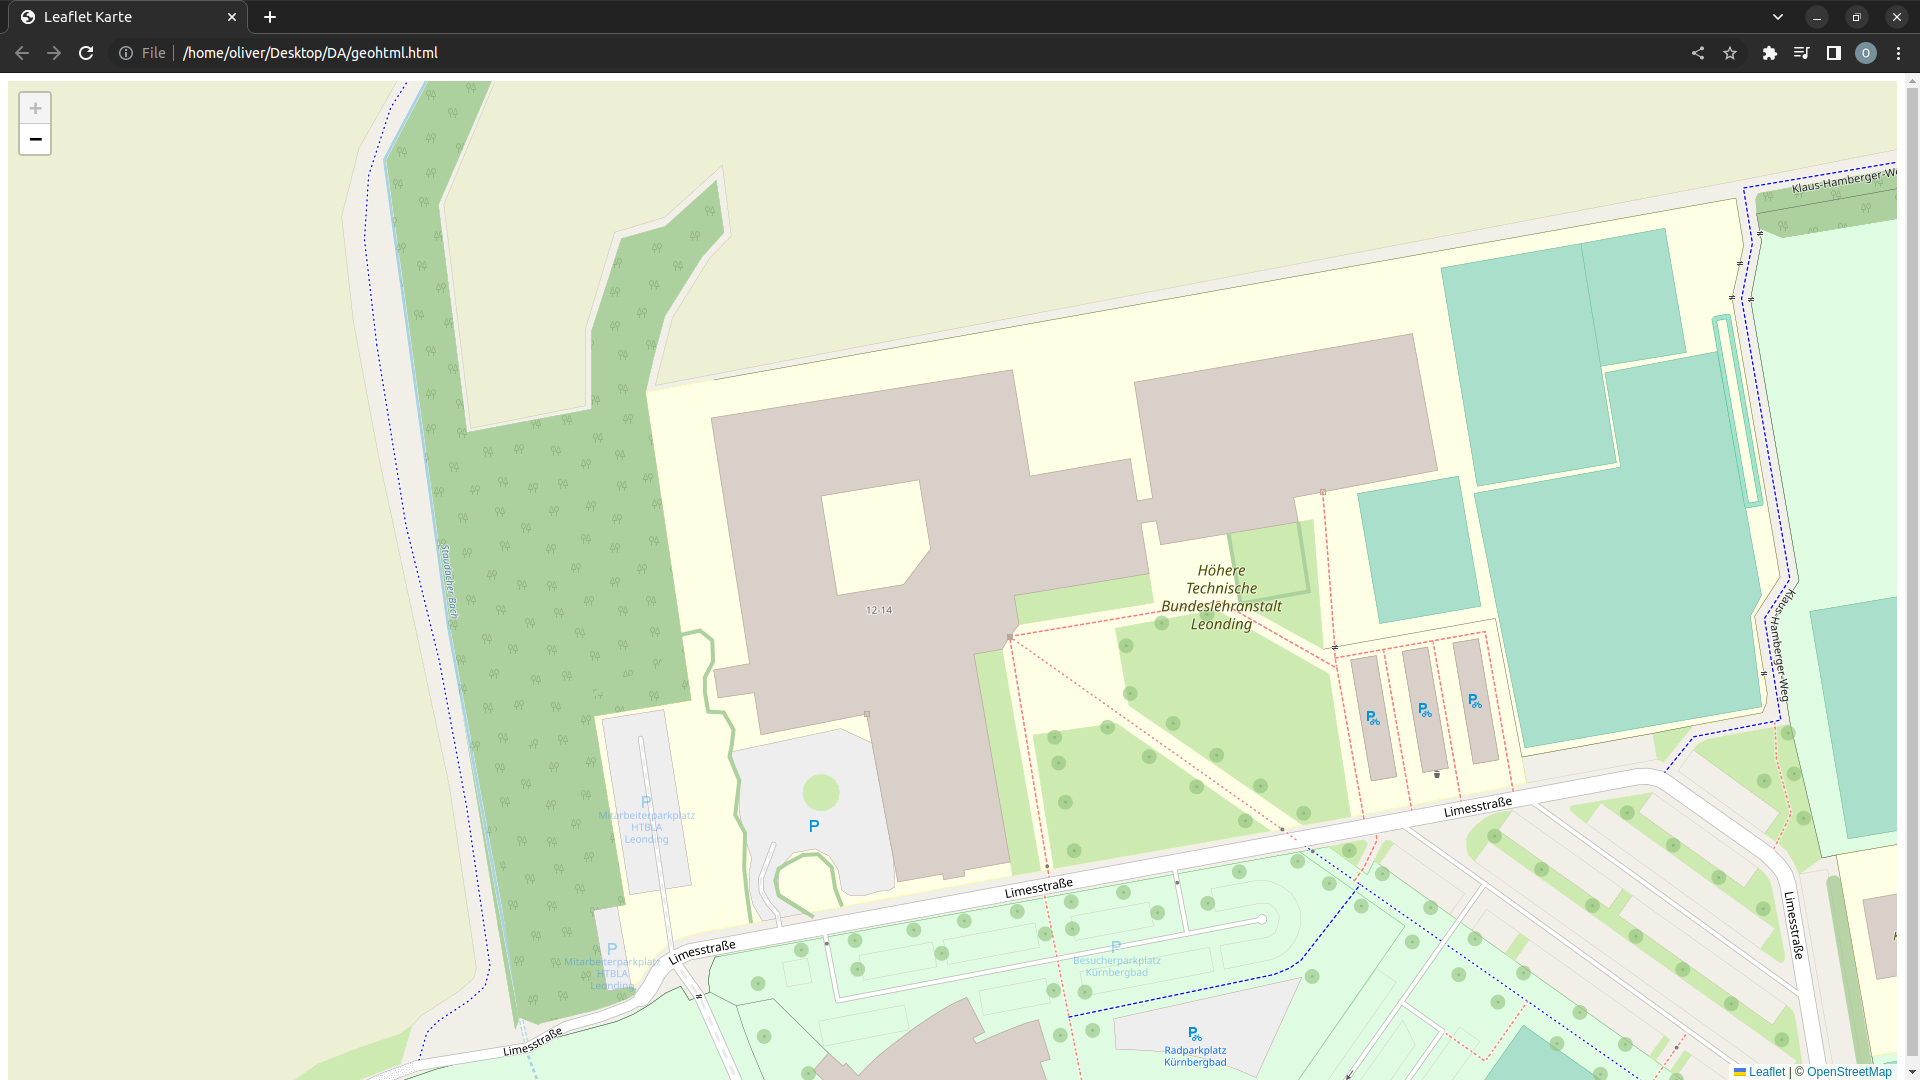
\includegraphics[scale=0.2]{pics/leafletmap.png}
\caption{Ergebnis der Implementierung mit Leaflet}
\end{figure}


\subsection{Version 2: Leaflet Karte mit Routing}
\setauthor{Oliver Sugic}
\cite{Liedman2015}Nach dem ersten Prototypen mit Leaflet, wurde die Idee weiter verfolgt, um die Benutzerfreundlichkeit für die Teilnehmenden zu verbessern. Eine Route vom eigenen Standort zur nächsten Aktivität wurde implementiert. Um die Routen anzeigen zu können, wurde die Leaflet Routing Machine verwendet. 
Hierfür wird das Plugin Leaflet Routing Machine verwendet, das ebenfalls vom Leaflet zur Verfügung gestellt wird. Mit dieser Erweiterung Können Routen zwischen zwei Punkten auf der Karte berechnet werden und angezeigt werden. Ebenfalls können die Wegpunkte einfach geändert werden.

\begin{lstlisting}[numbers=left,language=HTML,caption={Implementierung einer Karte mit Leaflet Routing Engine},label={lst:leafletmap}]
    <head>
    <title>Leaflet Karte</title>
    <style>
        #map {
            height: 1500px;
        }
    </style>
</head>

<body>
    <link rel="stylesheet" href="https://unpkg.com/leaflet@1.9.3/dist/leaflet.css"
        integrity="sha256-kLaT2GOSpHechhsozzB+flnD+zUyjE2LlfWPgU04xyI=" crossorigin="" />

    <script src="https://unpkg.com/leaflet@1.9.3/dist/leaflet.js"
        integrity="sha256-WBkoXOwTeyKclOHuWtc+i2uENFpDZ9YPdf5Hf+D7ewM=" crossorigin="">
        </script>
    <link rel="stylesheet" href="https://unpkg.com/leaflet@1.2.0/dist/leaflet.css" />
    <link rel="stylesheet" href="https://unpkg.com/leaflet-routing-machine@latest/dist/leaflet-routing-machine.css" />
    <script src="https://unpkg.com/leaflet@1.2.0/dist/leaflet.js"></script>
    <script src="https://unpkg.com/leaflet-routing-machine@latest/dist/leaflet-routing-machine.js"></script>

    <div id="map"></div>
    <script>
        var map = L.map('map').setView([48.2684159, 14.2517532], 15);
        L.tileLayer('https://tile.openstreetmap.org/{z}/{x}/{y}.png', {
            maxZoom: 19,
            attribution: '&copy; <a href="http://www.openstreetmap.org/copyright">OpenStreetMap</a>'
        }).addTo(map);
        L.Routing.control({
            waypoints: [
                L.latLng(48.2684159, 14.2517532),
                L.latLng(48.2627373, 14.2589871)
            ]
        }).addTo(map);
    </script>
\end{lstlisting}
\begin{figure}[h]
    \centering
    \includegraphics[scale=0.2]{pics/Leaflet_Routing.png}
    \caption{Ergebnis der Implementierung mit Leaflet Routing Machine}
\end{figure}

Allerding traten bei der Implementierung Probleme auf. Das Plugin konnte allerdings nicht die Route darstellen, was auf einen Fehler in der Implementierung zurückzuführen war.

\subsection{Version 3: Angular Geoloaction API}
\setauthor{Oliver Sugic}
Nach dem Scheitern der Implementierung mit der Leaflet Routing Machine, wurde eine neues Design entworfen, um die Benutzerfreundlichkeit zu verbessern.
Nach vielen Überlegung wurde ein Wireframe entworfen \ref{lst:Wireframe}, welches sowohl für mobile Endgeräte geeignet ist, aber auch überschaubar für die nutzenden Personen ist.

\begin{figure}[h]
    \centering
    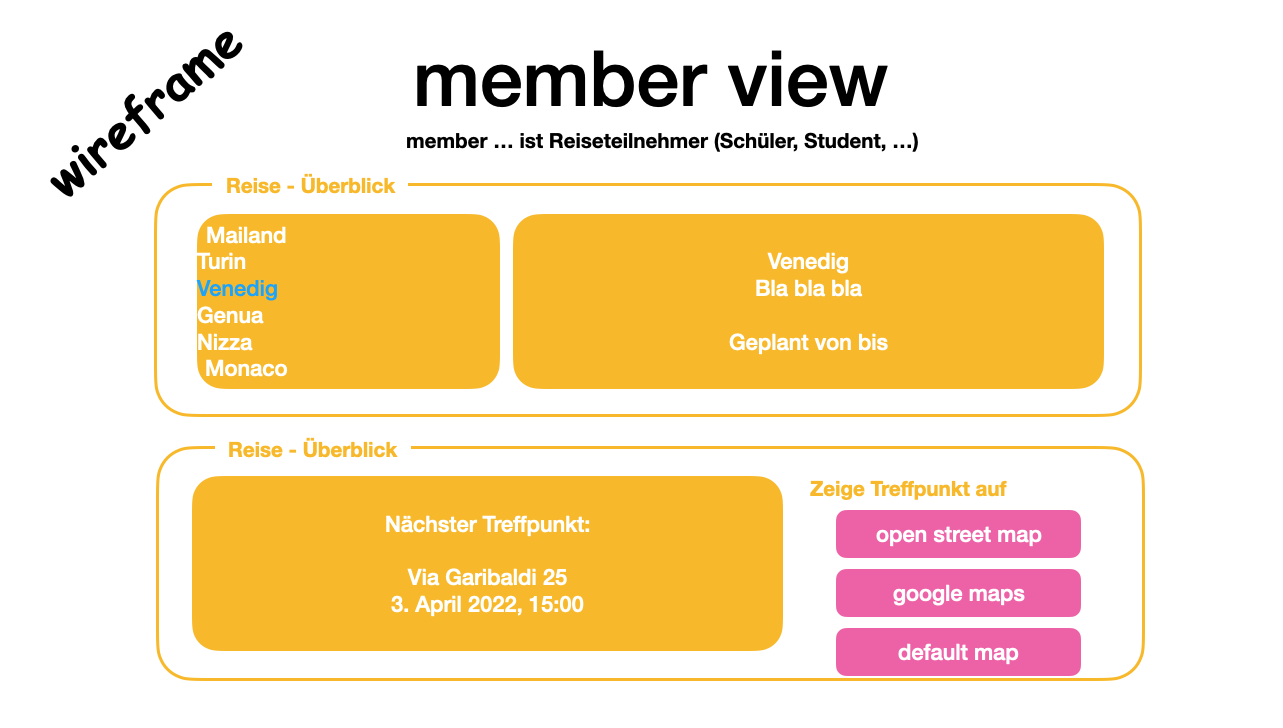
\includegraphics[scale=0.2]{pics/Wireframe.png}
    \caption{Endgültige Version }
    \label{lst:Wireframe}
\end{figure}

Der Nutzer soll in einen groben Überblick haben, welche Städte er besuchen wird. Durch eine kurze Beschreibung der Aktivität solle der Reisende einen kurzen Einblick haben, was Ihn erwarten wird. In der unteren Hälfte des Bildschirm erhält man genauere Informationen über den Treffpunkt, außerdem ist es möglich sich auf der Karte die Route anzeigen zu lassen. Es ist möglich, sich auf der standartmäßigen Karte des Endgeräts, über Google Maps oder über die OpenStreetMap zu navigieren. Der Nutzende kann für sich entscheiden, welche Karte Ihm am besten gefällt oder welche Karte Ihm am meisten vertraut ist. 

\section{Aktuelle Komponenten}
\setauthor{Oliver Sugic}
Derzeit besteht die Anwendung aus drei Komponenten. In diesem Kapitel werden der Aufbau und und Zusammenhänge der einzelnen Komponenten erläutert.  


\subsection{Angular Frontend}
\setauthor{Oliver Sugic}

Der schwierigste Teil der Arbeit liegt in darin, eine Benutzeroberfläche zu erstellen, die einfach zu bedienen aber auch ansprechend für den Benutzer ist.


\subsection{Quarkus Backend }
\setauthor{Oliver Sugic}

\subsection{Keycloak}
\setauthor{Oliver Sugic}

\subsection{Mögliche zukünftige Erweiterungen}
\setauthor{Oliver Sugic}




\begin{spacing}{1}
\chapter{Schnittstellendefinition}\label{chapter:tech}
\end{spacing}
\section{Beispiel}
\setauthor{Oliver Sugic}

\subsection{Erstellen eines Events}
\setauthor{Oliver Sugic}

\section{Rest-Endpoints}
\setauthor{Oliver Sugic}

\subsection{Create Event}
\setauthor{Oliver Sugic}

\subsection{Get Event By ID}
\setauthor{Oliver Sugic}
    
\subsection{List All Events}
\setauthor{Oliver Sugic}
    

\begin{spacing}{1}
\chapter{Ausgewählte Aspekte}\label{chapter:implementation}
\end{spacing}
\section{Standorterkennung durch Angular und Browser}
\setauthor{Oliver Sugic}


\section{Die Schüler Ansicht}
\setauthor{Oliver Sugic}

\section{JsonManagedReference und JsonBackReference}
\setauthor{Oliver Sugic}
    


\begin{spacing}{1}
\chapter{Resümee}
\end{spacing}
Während der Umsetzung der Diplomarbeit habe den durch Umgang mit neuen Technologien vieles neu dazu lernen können. Auch bei der Planung und Realisierung konnte ich viele Erfahrungen für mich mitnehmen. Blöderweise konnten das Projekt in ganzen unseren Vorstellung umgesetzt werden, das es seitens meiner Diplomarbeitspartner nicht mehr weiter verfolgt wurde. Das Projekt ist durchaus gut gelungen, für die harte Arbeit, die ich investiert habe.


\newpage
\pagenumbering{Roman}
\setcounter{page}{\value{RPages}}
\newacronym{guid}{GUID}{Globally Unique Identifier}
\newacronym{jit}{JIT}{Just In Time Compiler}
\newacronym{nfc}{NFC}{Near Field Communication}
\newacronym{rfid}{RFID}{Radio Frequency Identification}

% Usage:
% \gls{label} lowercase in text
% \Gls{label} Uppercase in text
% \newacronym{label}{abbrev}{full}
% \newglossaryentry{label}{settings}



%\setlength{\glsdescwidth}{0.8\linewidth}
\glsnogroupskiptrue
\printglossary[title=Glossar,toctitle=Glossar] %,style=long]
\spacing{1}{
%\bibliographystyle{IEEEtran}
\bibliographystyle{ieeetrande}
\bibliography{bib}
}
\listoffigures
\listoftables
\lstlistoflistings
\appendix
\addchap{Anhang}
%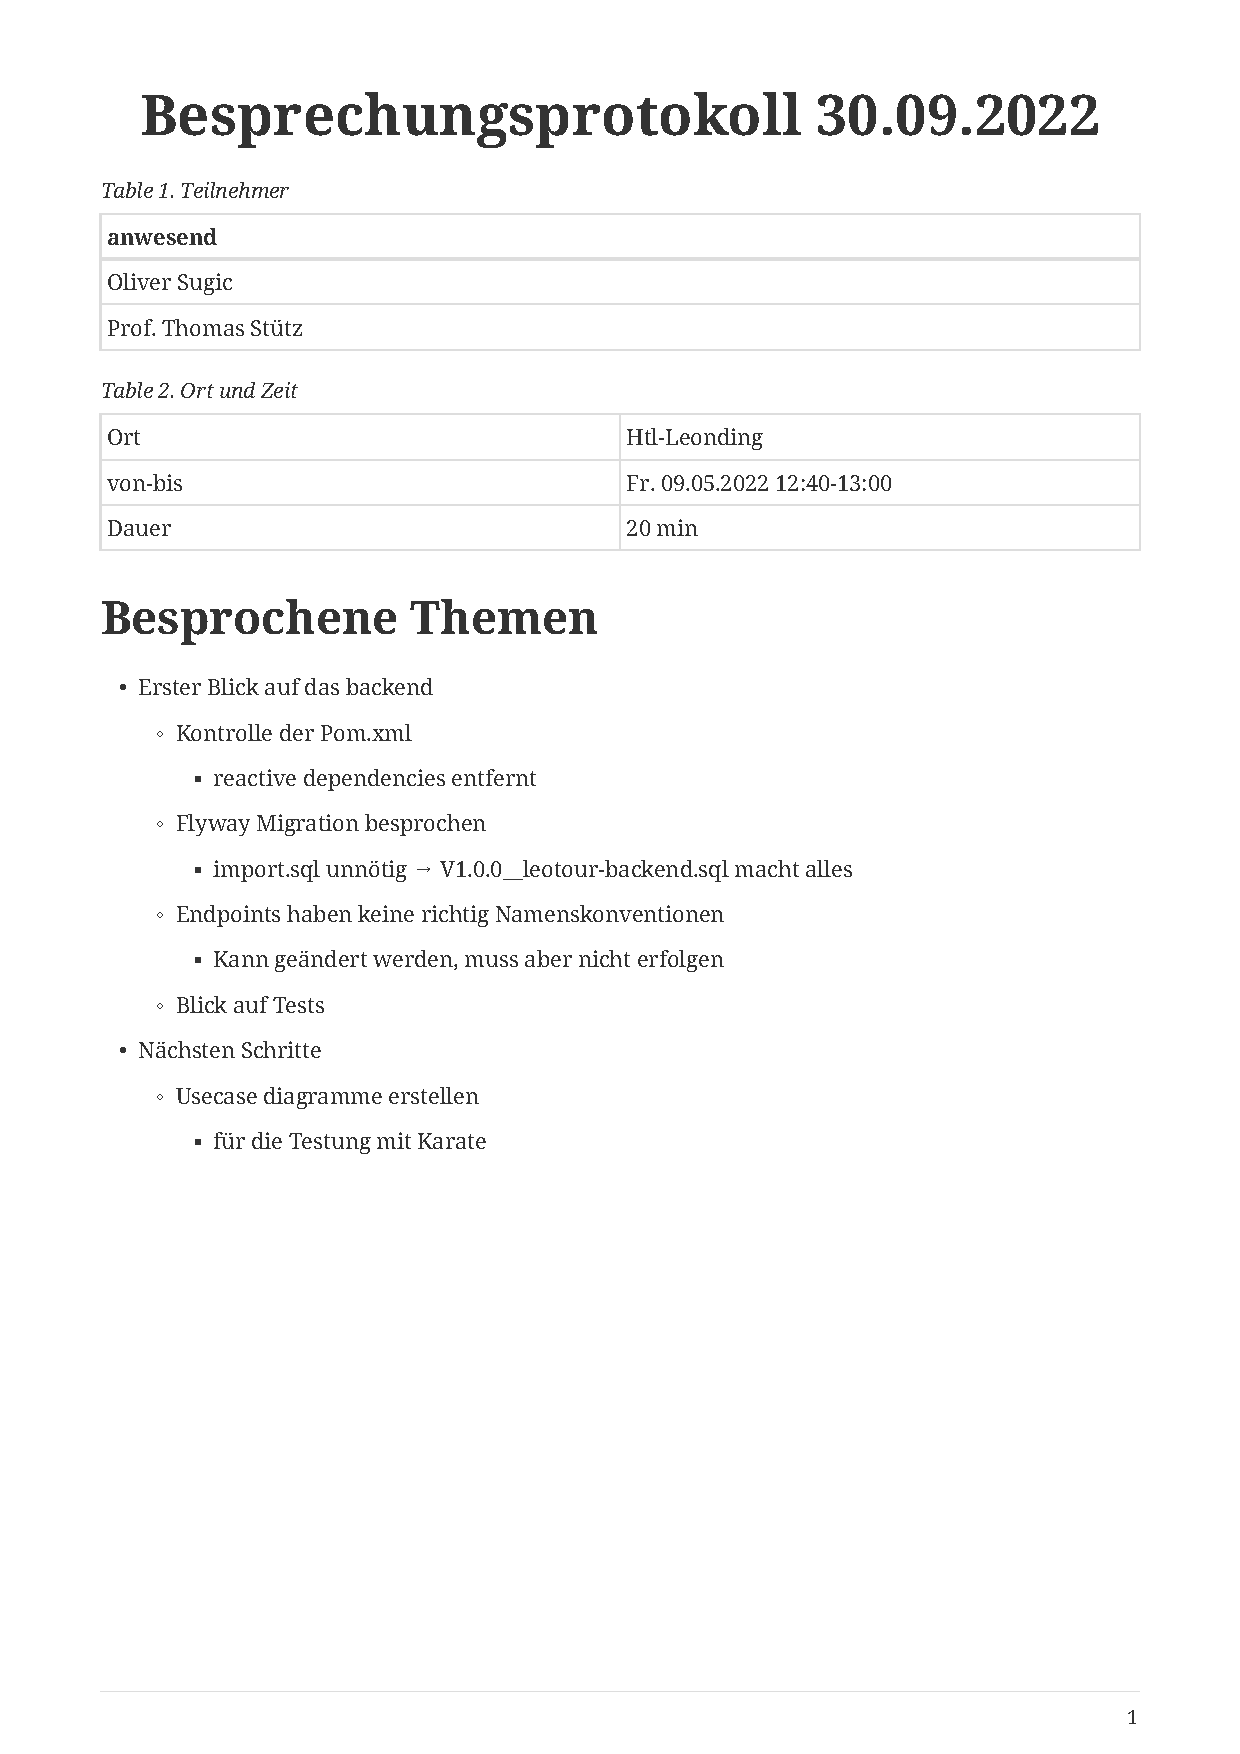
\includepdf[scale=0.9]{MoM/minutes-of-meeting-2022-09-30.pdf}
%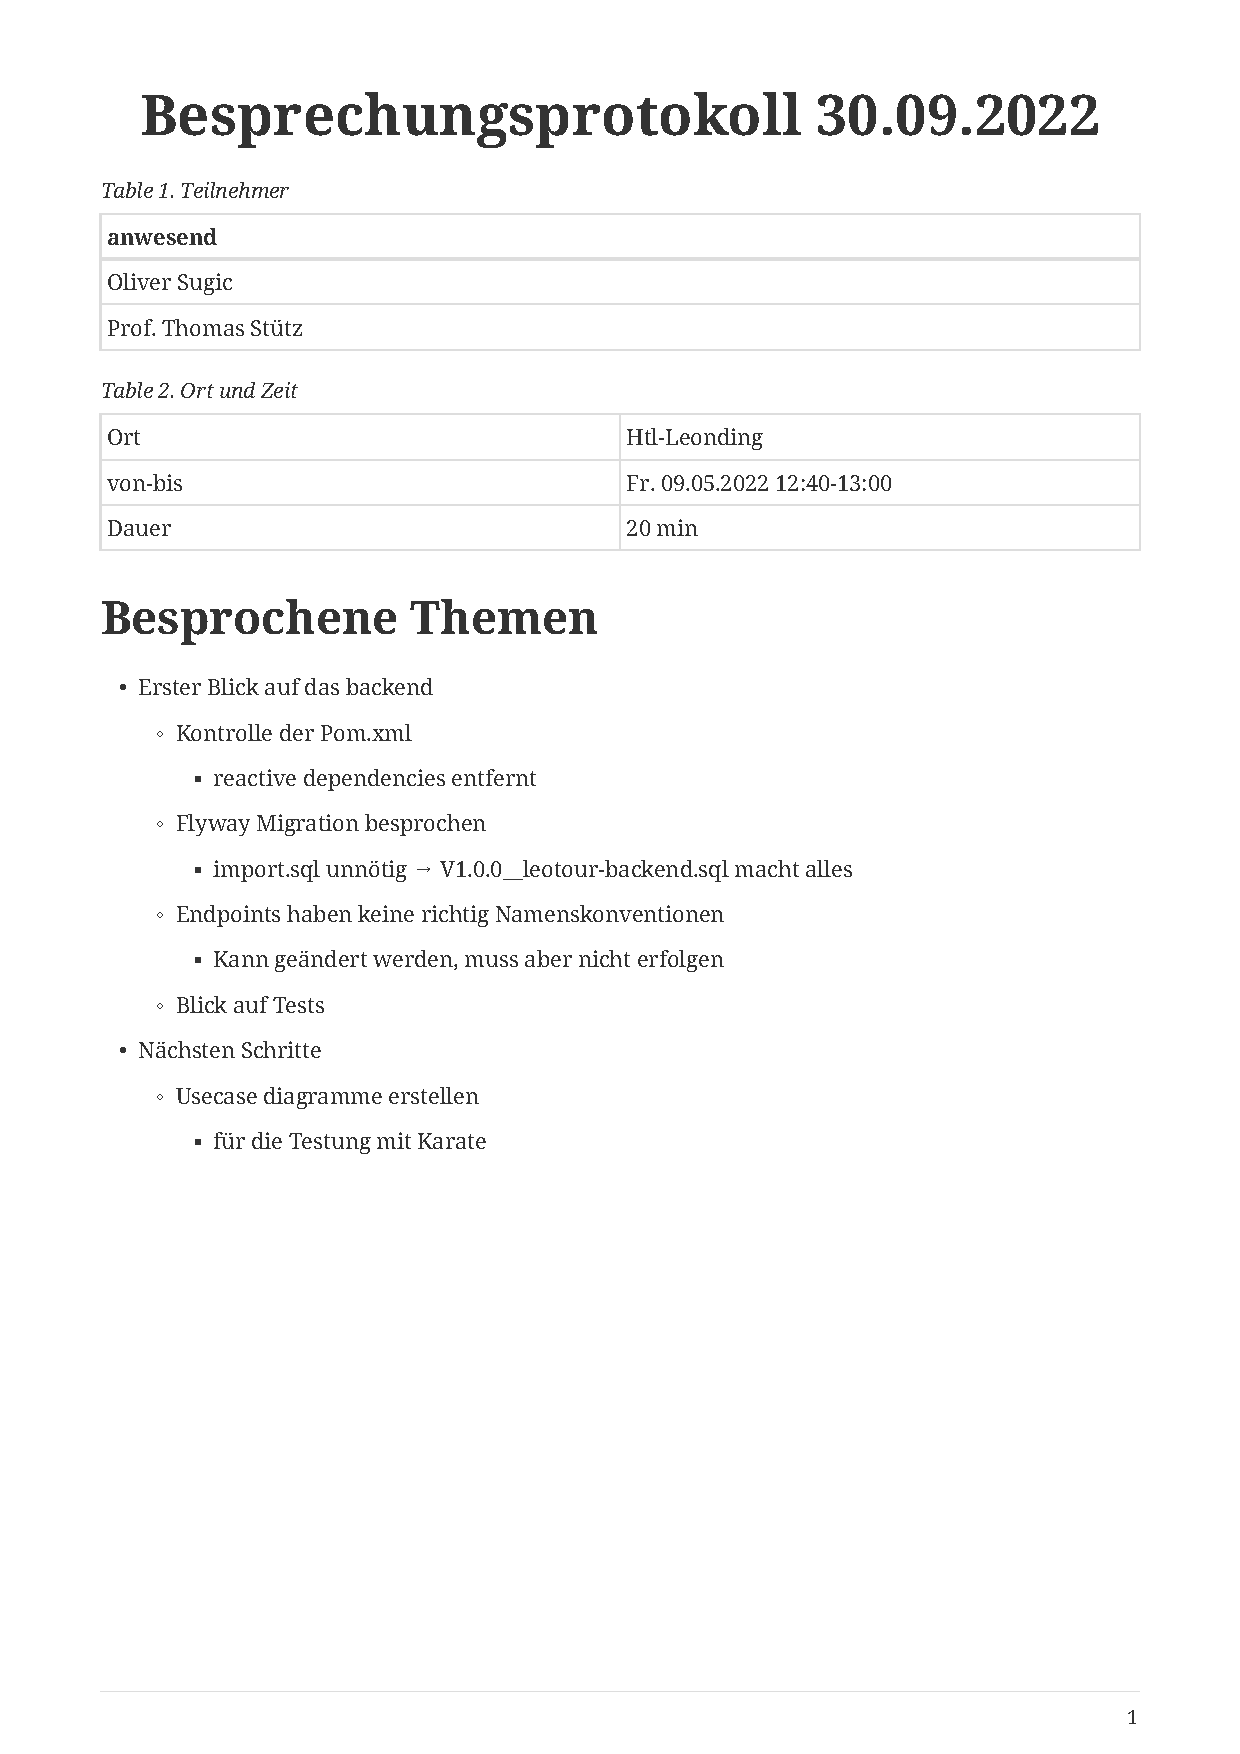
\includepdf[scale=0.7,pagecommand={}]{MoM/minutes-of-meeting-2022-09-30.pdf}
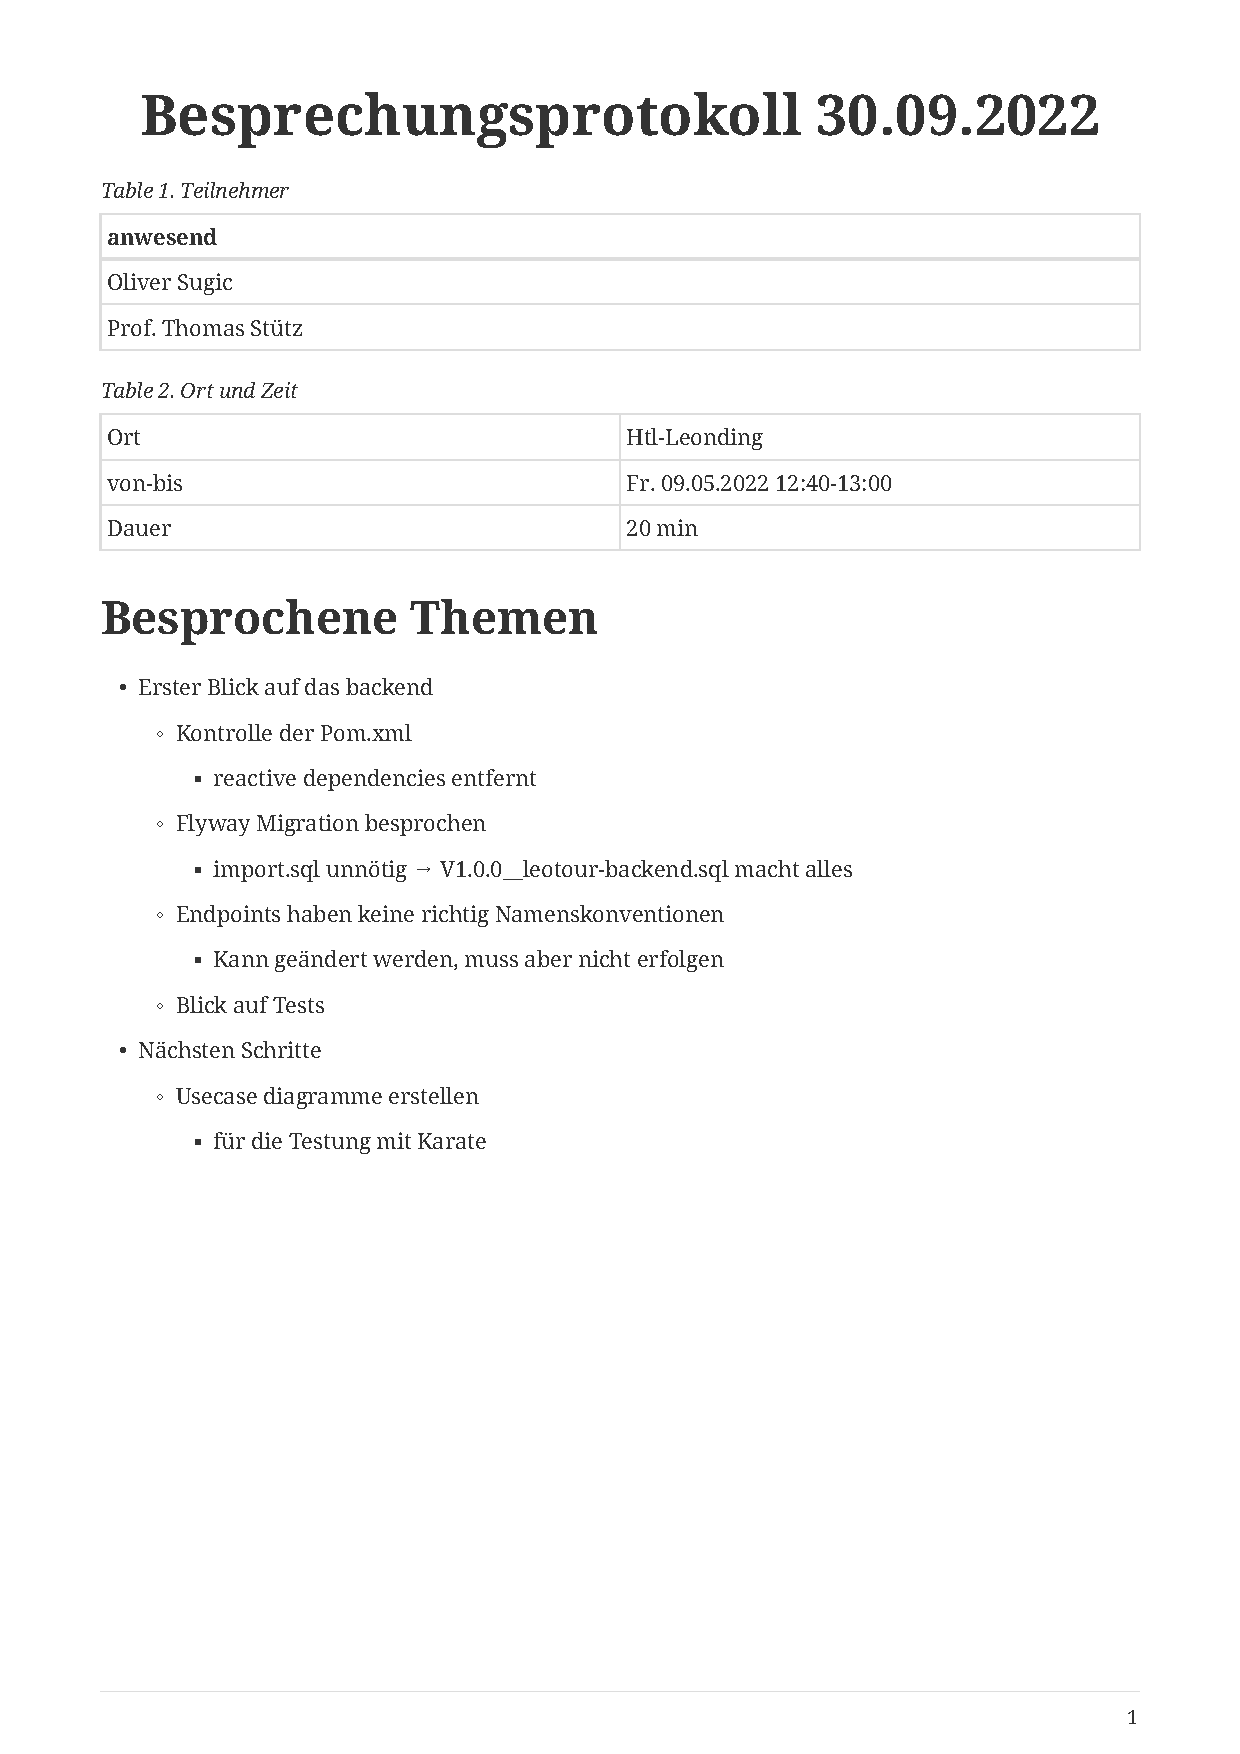
\includepdf[pages=1,scale=0.85]{MoM/minutes-of-meeting-2022-09-30.pdf}
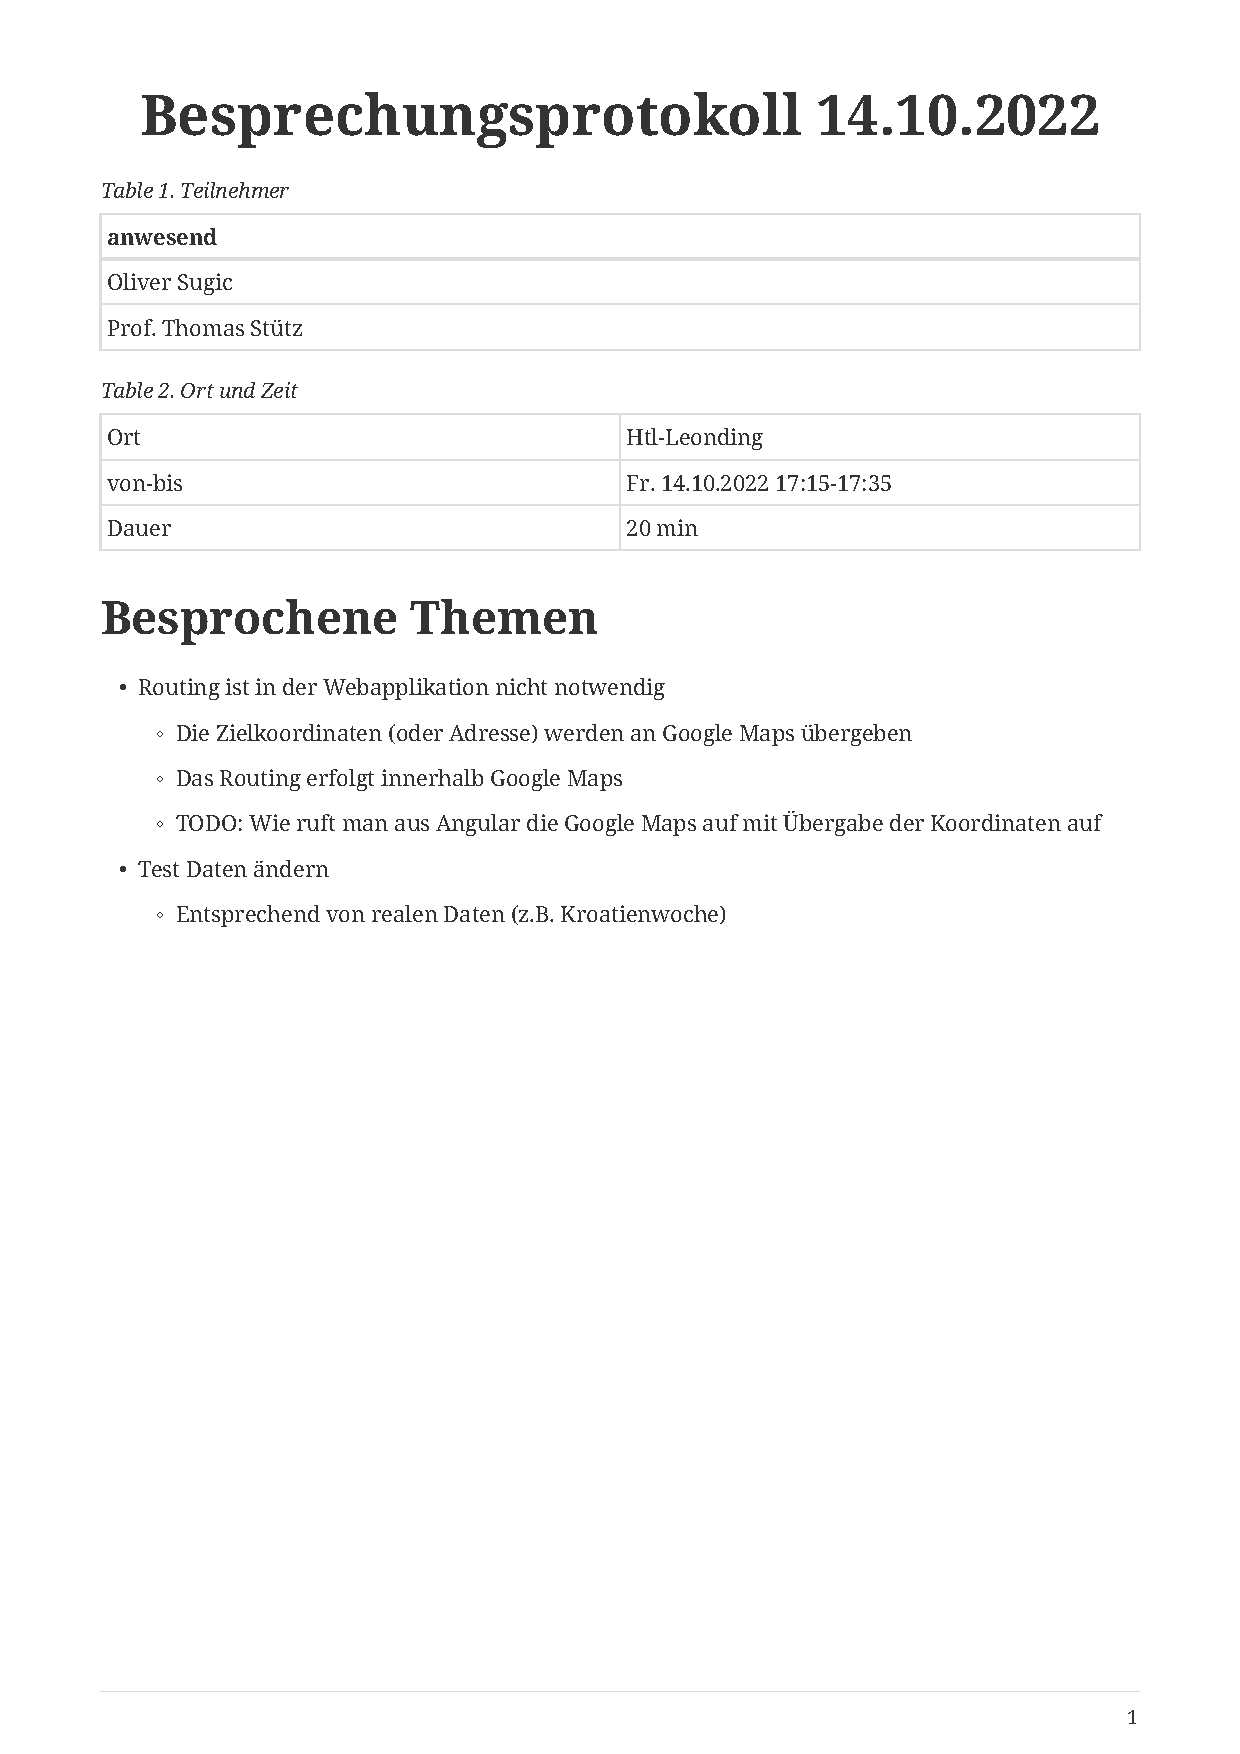
\includepdf[pages=1,scale=0.85]{MoM/minutes-of-meeting-2022-10-14.pdf}
\includepdf[pages=2,scale=0.85]{MoM/minutes-of-meeting-2022-10-23.pdf}
\end{document}